\subsection{Periodic Background Tasks}\label{ssec:periodictasks}
When the app is installed on the device, the app needs to run a task to periodically collect location data.
\Citet{friesen2015android} writes how this can be done in the Android API by utilizing the AlarmManager and the JobSchedular.

\textbf{AlarmManager}\\
The AlarmManager was created to handle alarms, and implemented as a general class that can call any task after one or multiple given time periods.
The alarm can be set to be reoccurring, thus gather a location with the given interval.

\textbf{JobScheduler}\\
The JobScheduler was implemented in Android 5.0 (API 21) as an alternative to the AlarmManager.
The scheduler behaves in a similar way as the AlarmManager, but tries to batch the jobs together and execute them in bundles.
This means that the device can save power by avoiding going to sleep just to wake a short moment later, on the cost of time precision. 
While the AlarmManager has the option to occur at a exact time, the JobSchedular does not.

The JobScheduler is chosen as the basis for the background tasks, because the timing accuracy of the location data is not sensitive to minor deviations, in addition to the advantages of saving power features.

\subsection{Location tracking}\label{ssec:loctrack}
% metatext
In order to be able to locate a user and to construct routes, it is necessary to collect location data. 
Such collection of locations can be done by using already existing services, such as the Google Play Services.

% something
Location data in \gls{rs} is formatted in decimal coordinates in an array that represents a route from A to B.
There are several ways to collect location data. 
One of them is to manually develop a component to do so on the Android device, but the chosen solution is to utilize the already existing Google Play Services.

To use Google Play Services, a client library must be included in the app, and will communicate via inter-process communication to the Google Play Services. 

An advantage of the Google Play Services \cite{GapiOverview}, is that it will automatically receive silent updates regularly, to acquire new features and bug fixes to the used services, developed by Google, and this is illustrated in Figure \ref{fig:gapifigure}.
The Google Play Services are restricted, and are not supporting devices with Android versions lower than 2.3. 
This limits the backwards compatibility, but the app is already restricted to Android 5 and newer, and has no influence on the target audience.

\begin{figure}[h]
	\centering
	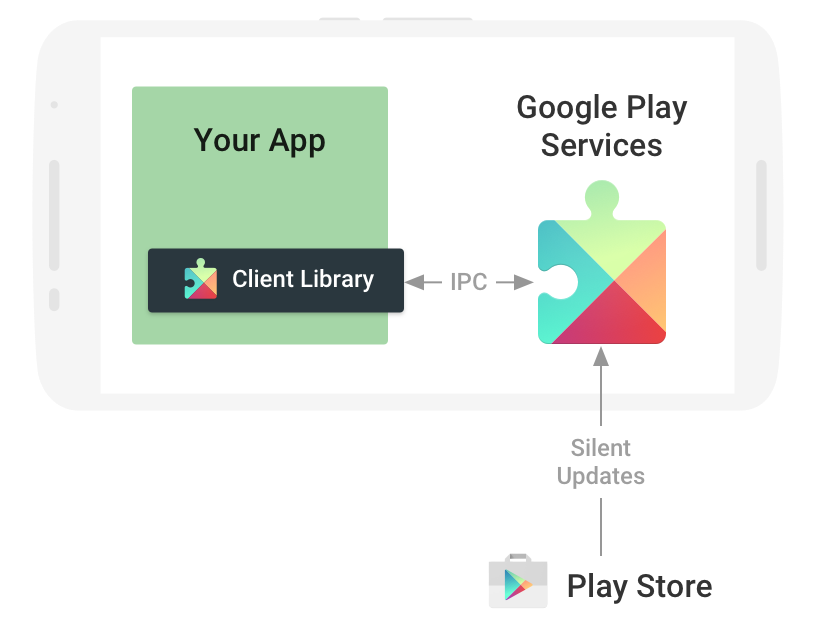
\includegraphics[width=0.7\textwidth]{figures/play-services-diagram.png}
	\caption{Google Play Services communication\cite{GapiFigure}}
	\label{fig:gapifigure}
\end{figure}

The Google Play Services will allow the app to collect location data, but it is not doing so solely by using the GPS in the device. 
The location service utilizes both network location and GPS to estimate a position as precise as possible \cite{GapiLocation}. 
To ensure the collected location data is relevant, locations are only collected when the user is traveling by vehicle.

The Google Play Services provides a service to determine the user's activity, called Activity recognition. 
Activity recognition is a service that utilizes several sensors on the device to determine what kind of activity the user is currently performing, therein driving, walking, etc. \cite{activitysensor}.
The service will return a probability level from 0 to 100, where 100 is certain that a user is performing the activity.
The activity recognition will also prevent unnecessary data will be stored on the database. 

The practical design of the location tracking and activity recognition will be further explored in the following design section.
The \gls{astep} system is examined as an external tool, and its functionalities are explored.